\chapter{Einleitung}

\chapter{Konzeption}
\label{ch:intro}
\section{Zielgruppe}
\label{sec:intro:motivation}

\graffito{Note: The content of this chapter is just some dummy text. It is not a real language.}

ZG sind primär Kunden, die überlegen die Drohne für suchaktionen einzusetzen.
somit sollen die Zuschauer am ende des Filmes eine konkrete idee haben, wie die drohne eingesetzt wird und mit welchem aufwand das ganze verbunden ist.
weiterhin soll der film optional auch für allgemein an dem Projekt Interessierte oder potenzielle Teammitglieder hilfreich sein

um dem Zuschauer zu unterbewusst zu vermitteln, wurde Videomaterial eingebaut. Da jedoch manche Prinzipien während dem Flug besser erklärt werden können, und hier 


\section{Outline des Filmes}
\label{sec:intro:goal}
es werden die 6 Stationen gezeigt:
1. Programmieren/Flugplan
2. Zusammenbau
3. Start
4. Flug
5. Landung
6. Auswertung

sodass der zuschauer ein umfassendes bild hat, wie die drohne eingesetzt wird, und welcher aufwand damit verbunden ist.

einfügen von rettungsfloß, um am ende den nutzen besser zeigen zu können
bzw. erfolg darstellen können

einfügen von intro und outro als ``Spange'' für den film
flug über wasser soll in bildsprache transportieren, wie hoffnungslos eine suche ist, da das mehr eine extreme weite hat


wiederkehrende bildsprache, so ist das segelboot schon am anfang sichtbar, dann springt die kamera dahin

genauso auch am ende vom flug, ist das segelboot schon sichtbar, von dem aus im nächsten Shot das flugzeug gesehen wird

\section{Animatic / layouting}
\label{sec:intro:structure}
segelboot und ein stark vereinfachtes modell vom flugzeug wurden als layouting benutzt
layouting diente dazu, herauszufinden was in welcher reihenfolge gezeigt wird
darüber hinaus wurde versucht zu jeder eigenschaft eine passende bildsprache zu finden
bspw steigt das flugzeug, währrend von der flughöhe gesprochen wird
oder die kamera fliegt leicht hinter dem flugzeug währrend von der fluggeschwindigkeit gesprochen wird

reihenfolge wurde dann noch einmal geändert weil ...?

\begin{figure}
\begin{tabular}{cc}
\subfloat[caption]{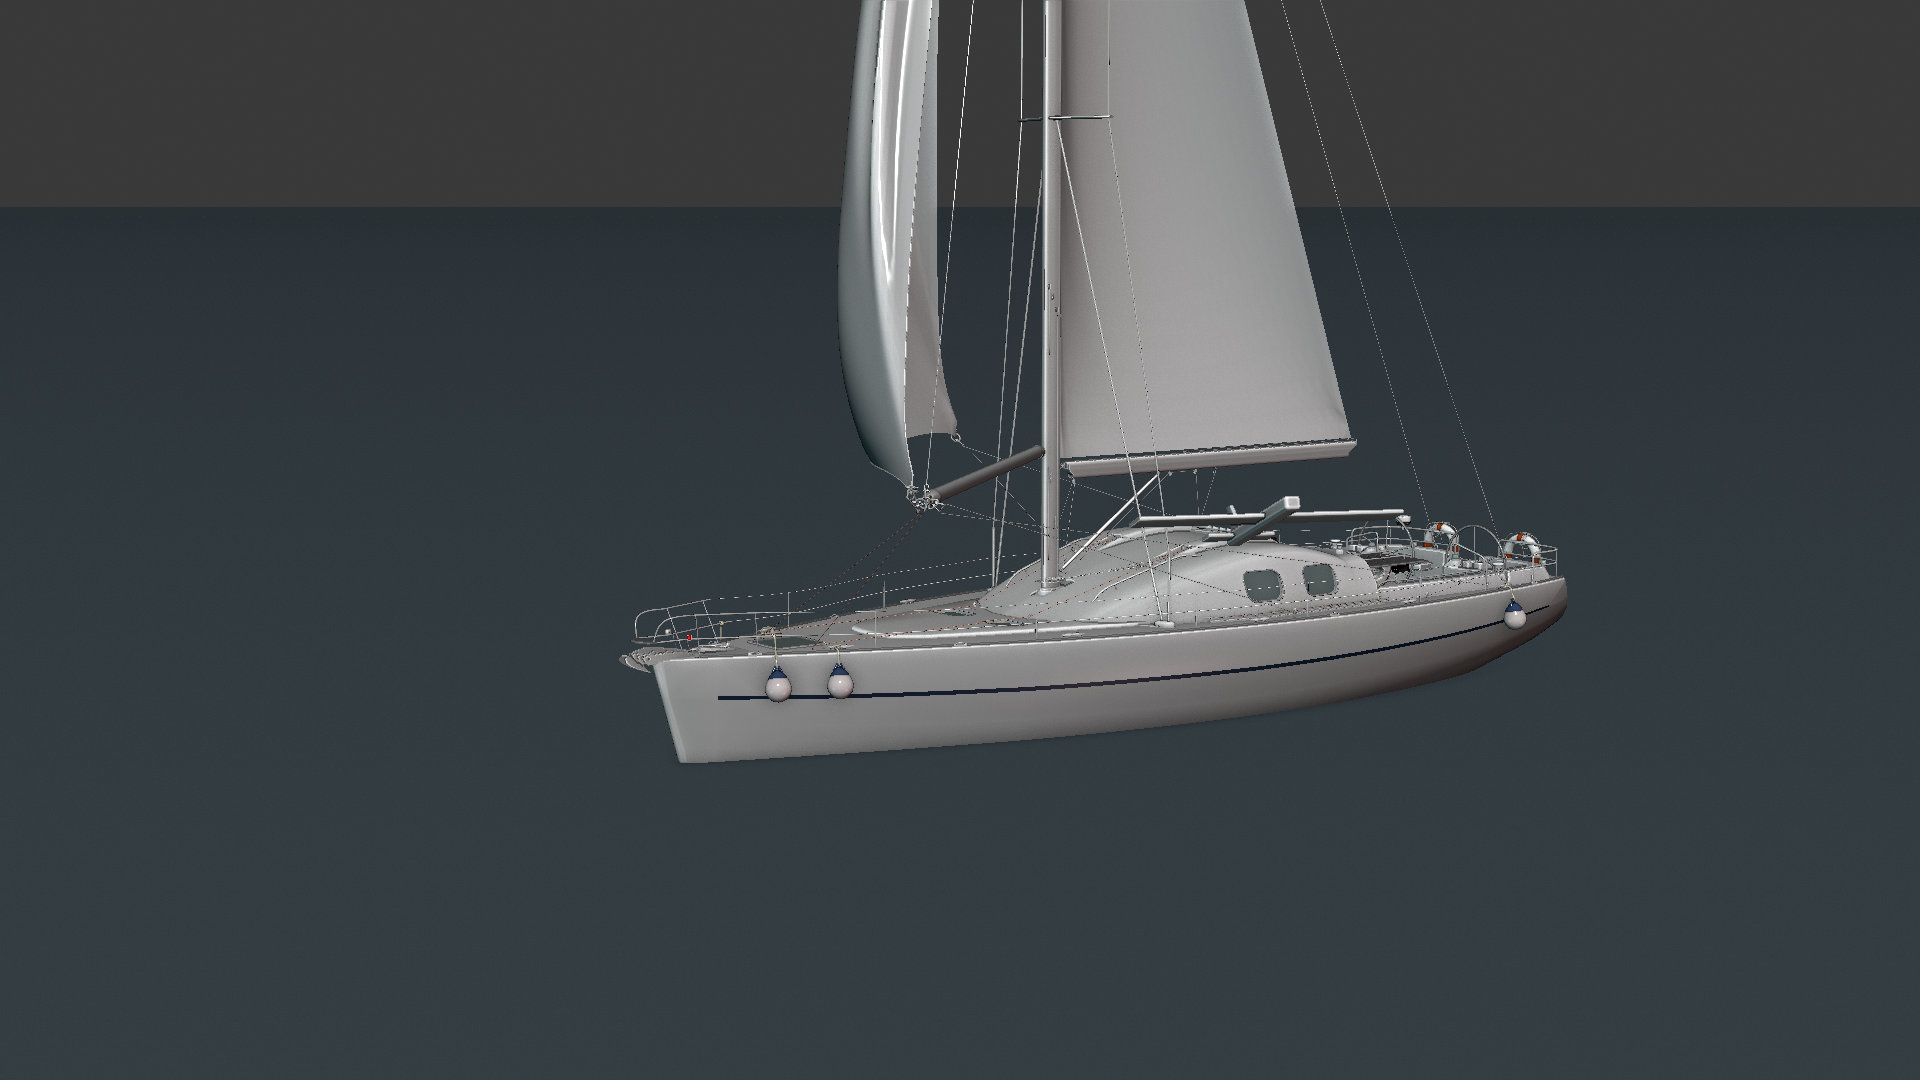
\includegraphics[width=\textwidth/2]{gfx/pre/0058.jpg}} &
\subfloat[caption]{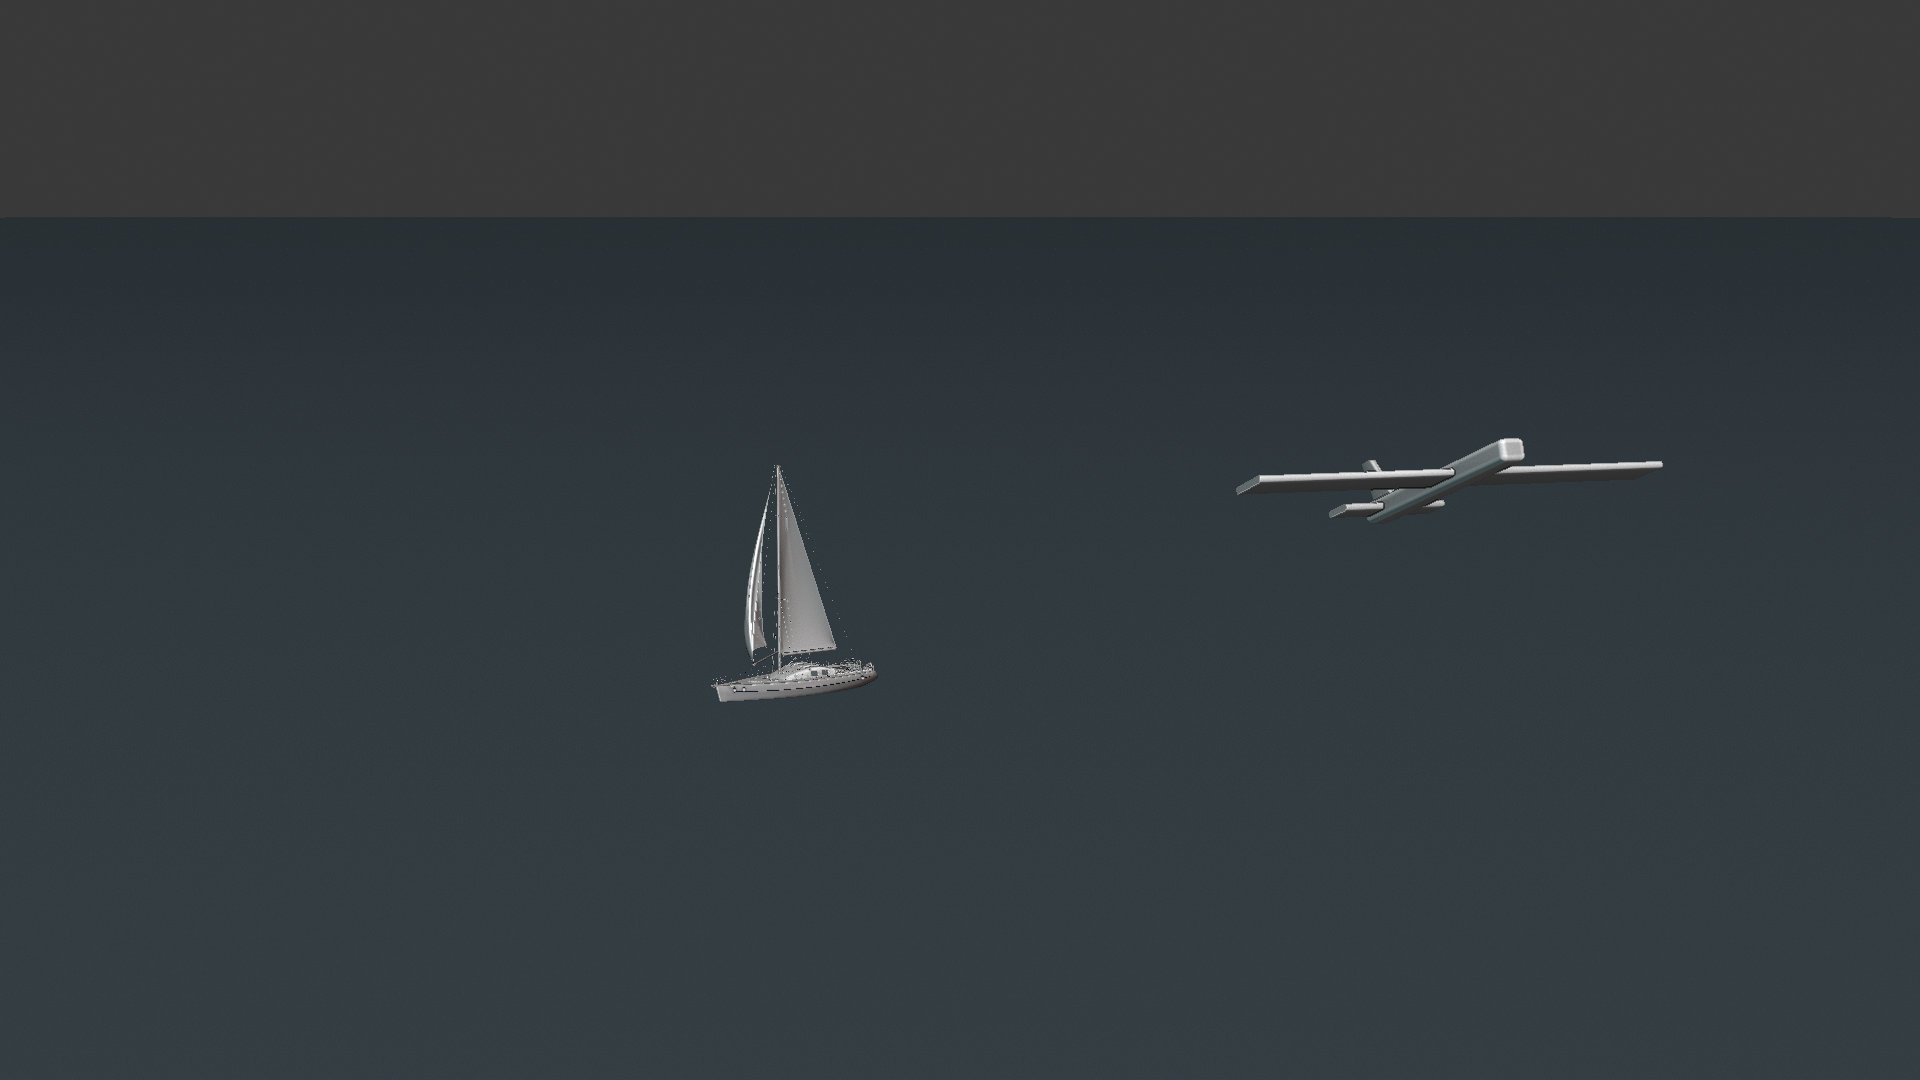
\includegraphics[width=\textwidth/2]{gfx/pre/0059.jpg}} \\
\subfloat[caption]{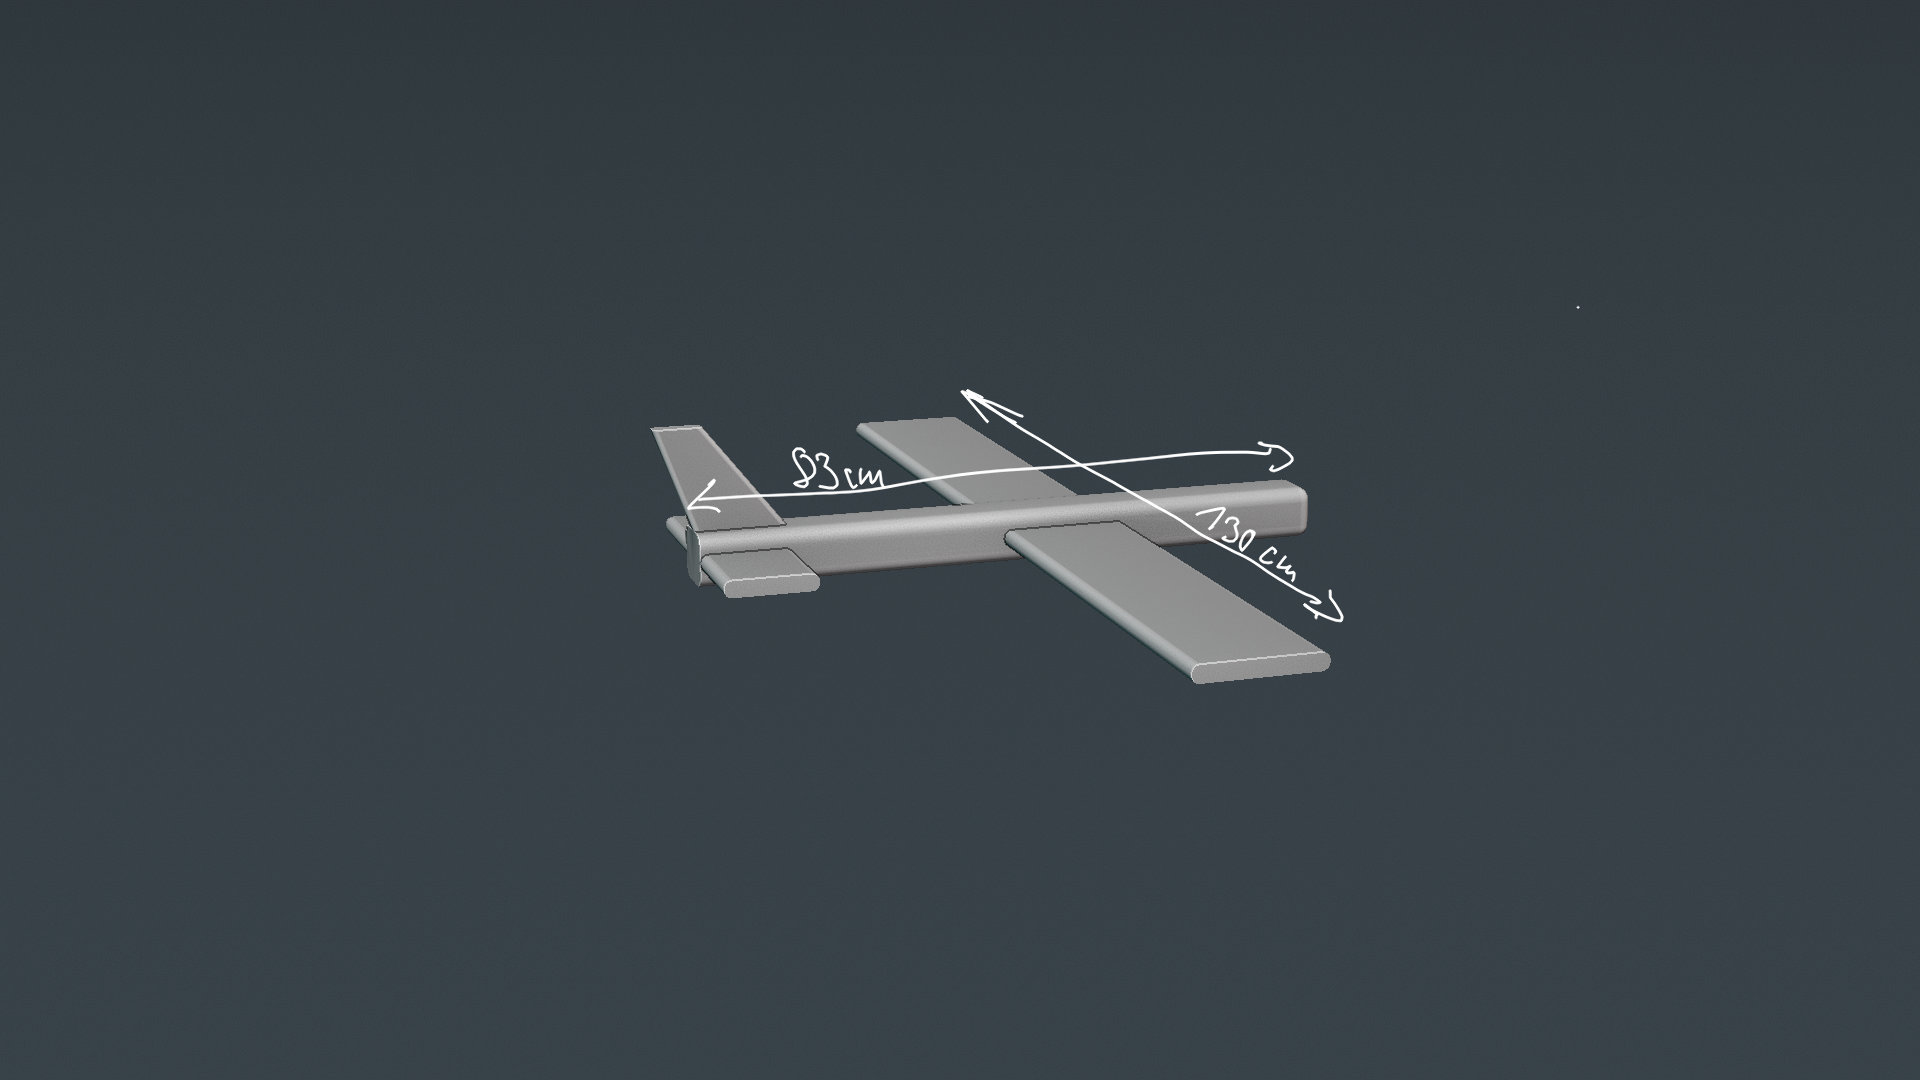
\includegraphics[width=\textwidth/2]{gfx/pre/0119.jpg}} &
\subfloat[caption]{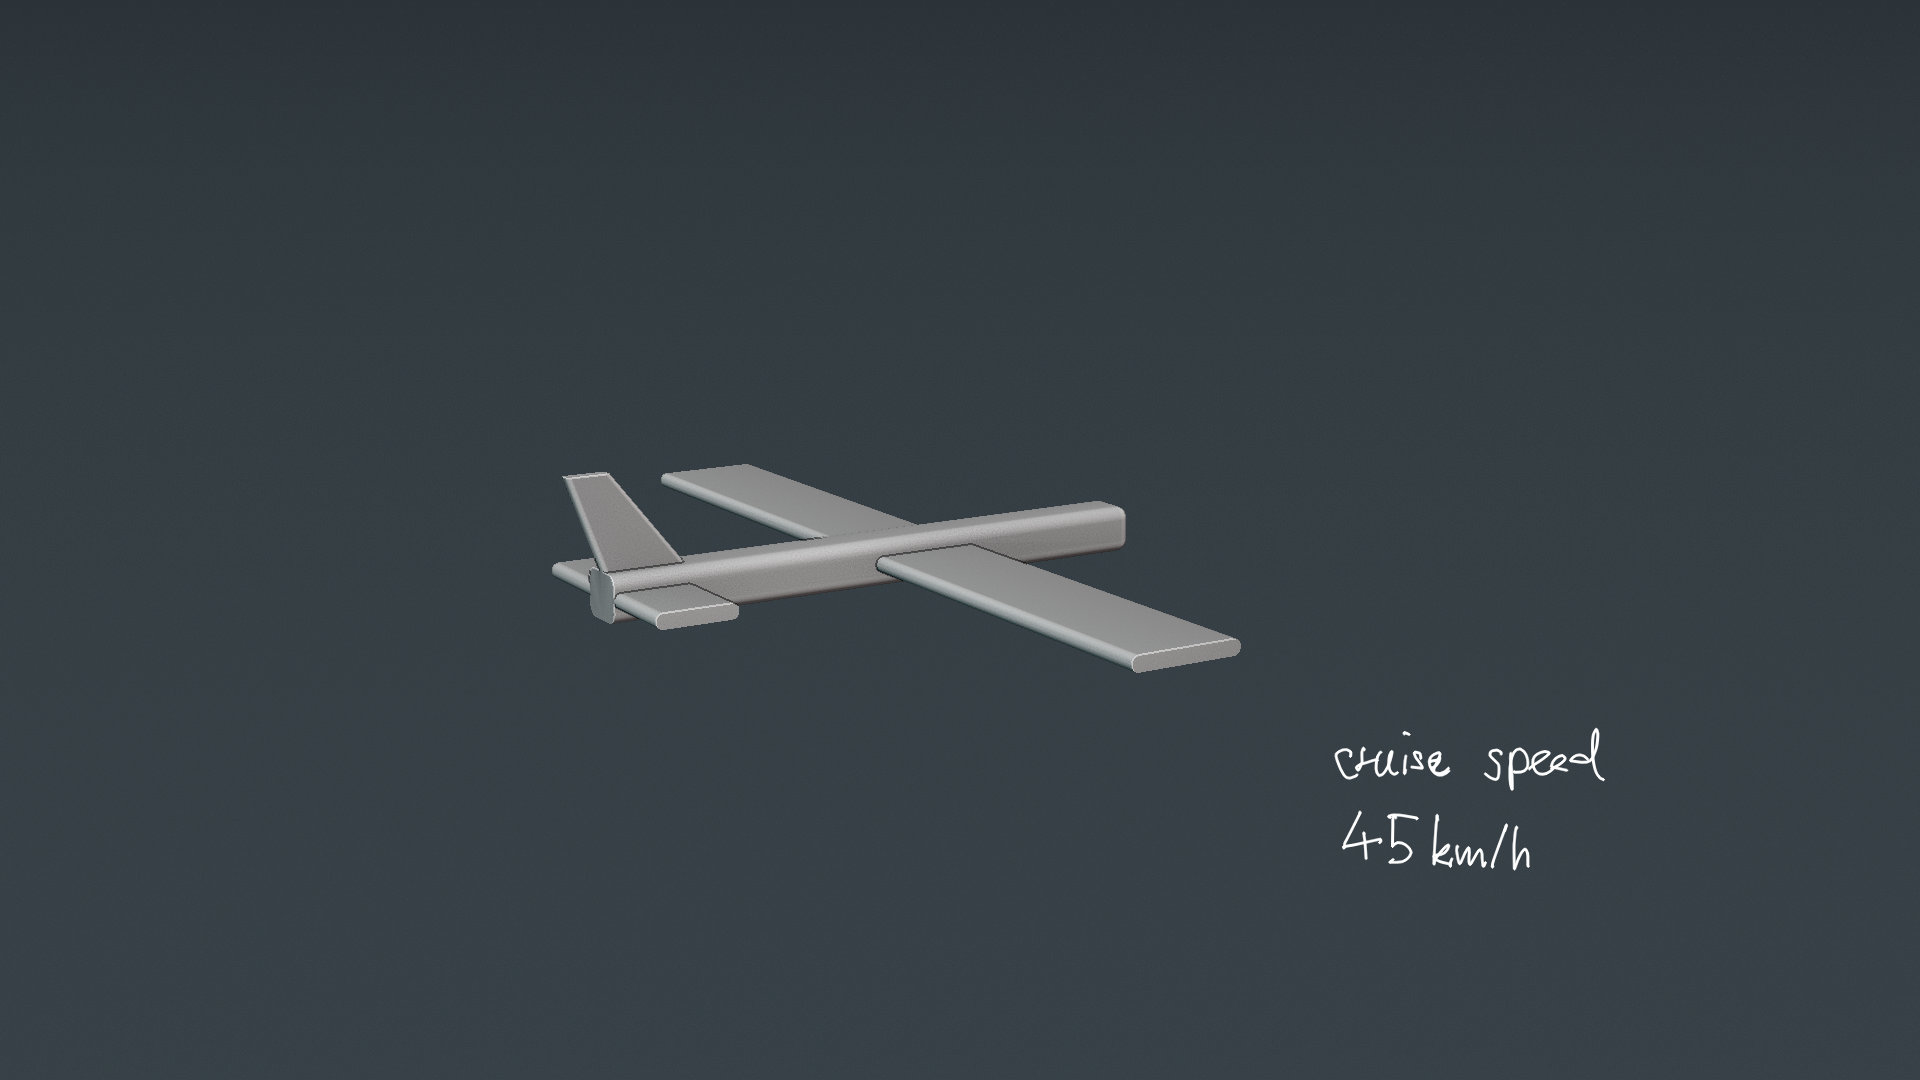
\includegraphics[width=\textwidth/2]{gfx/pre/0180.jpg}} \\
\subfloat[caption]{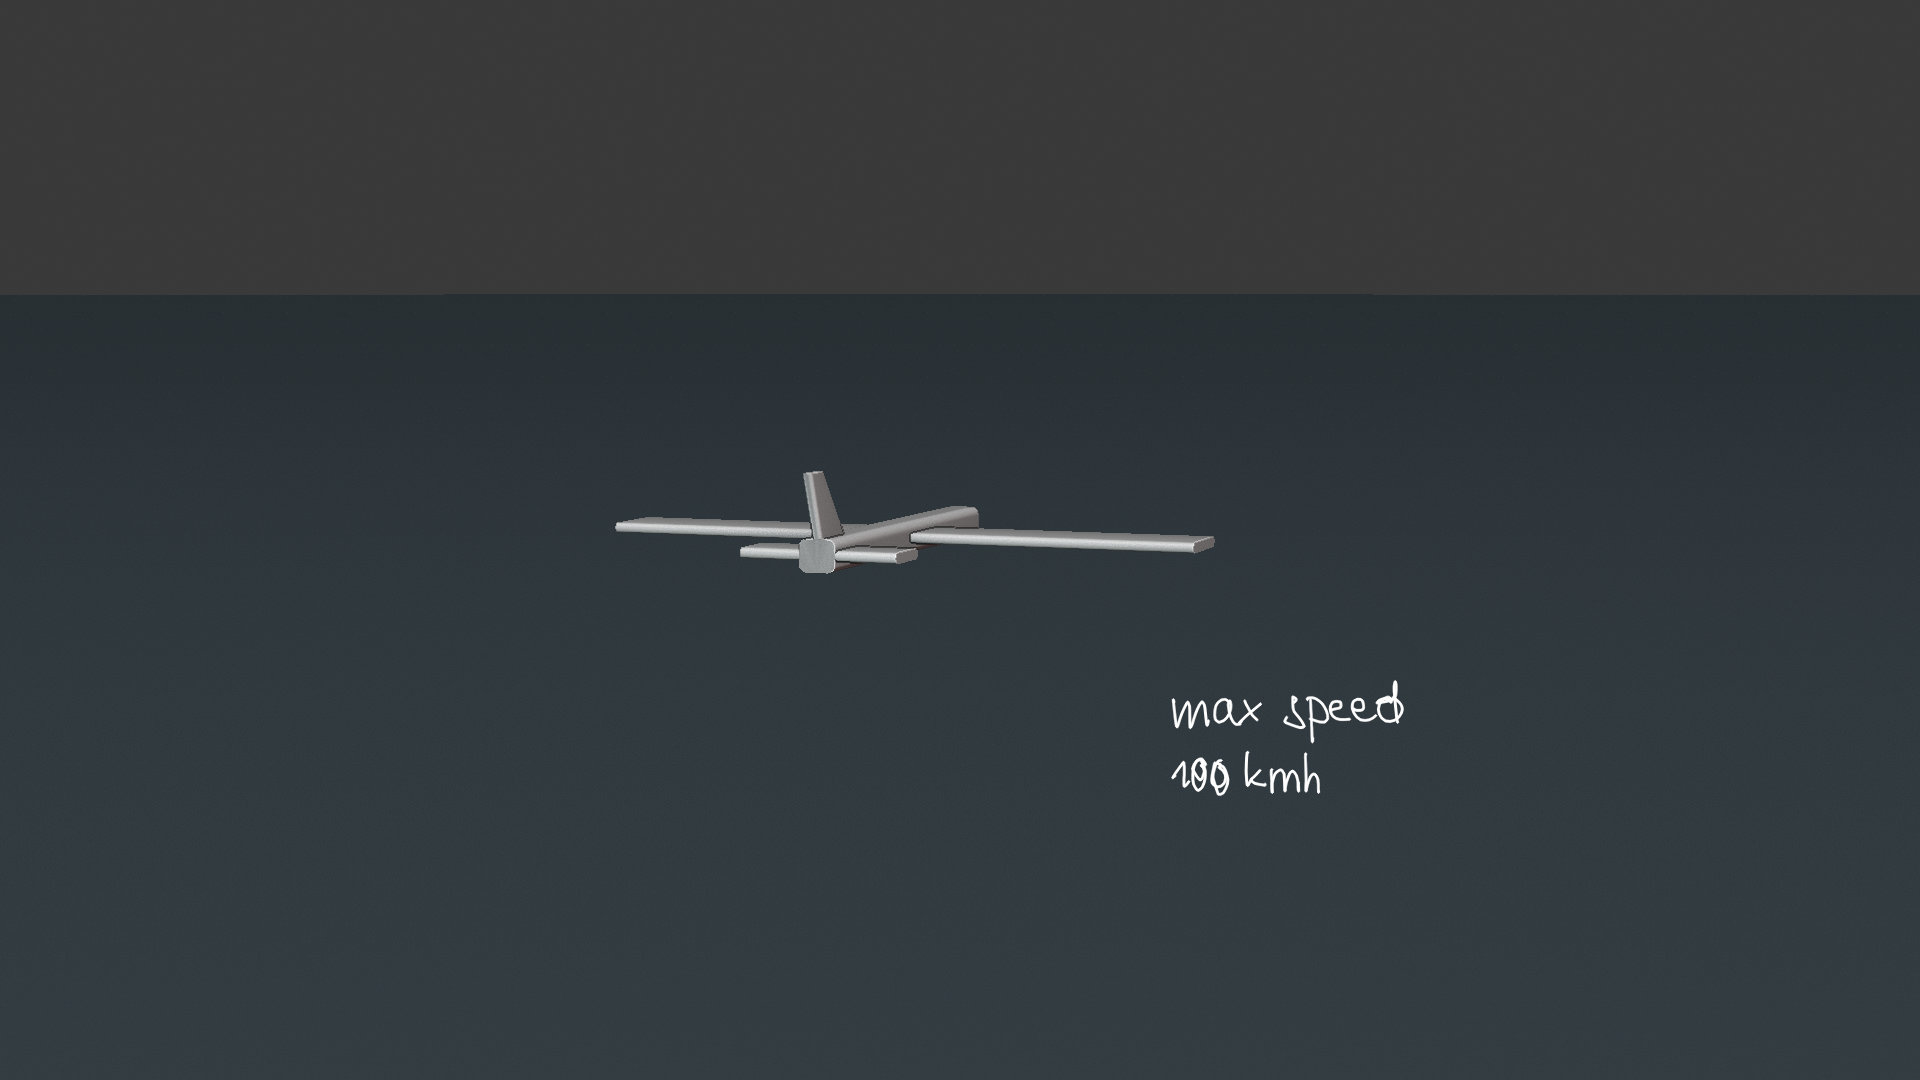
\includegraphics[width=\textwidth/2]{gfx/pre/0239.jpg}} &
\subfloat[caption]{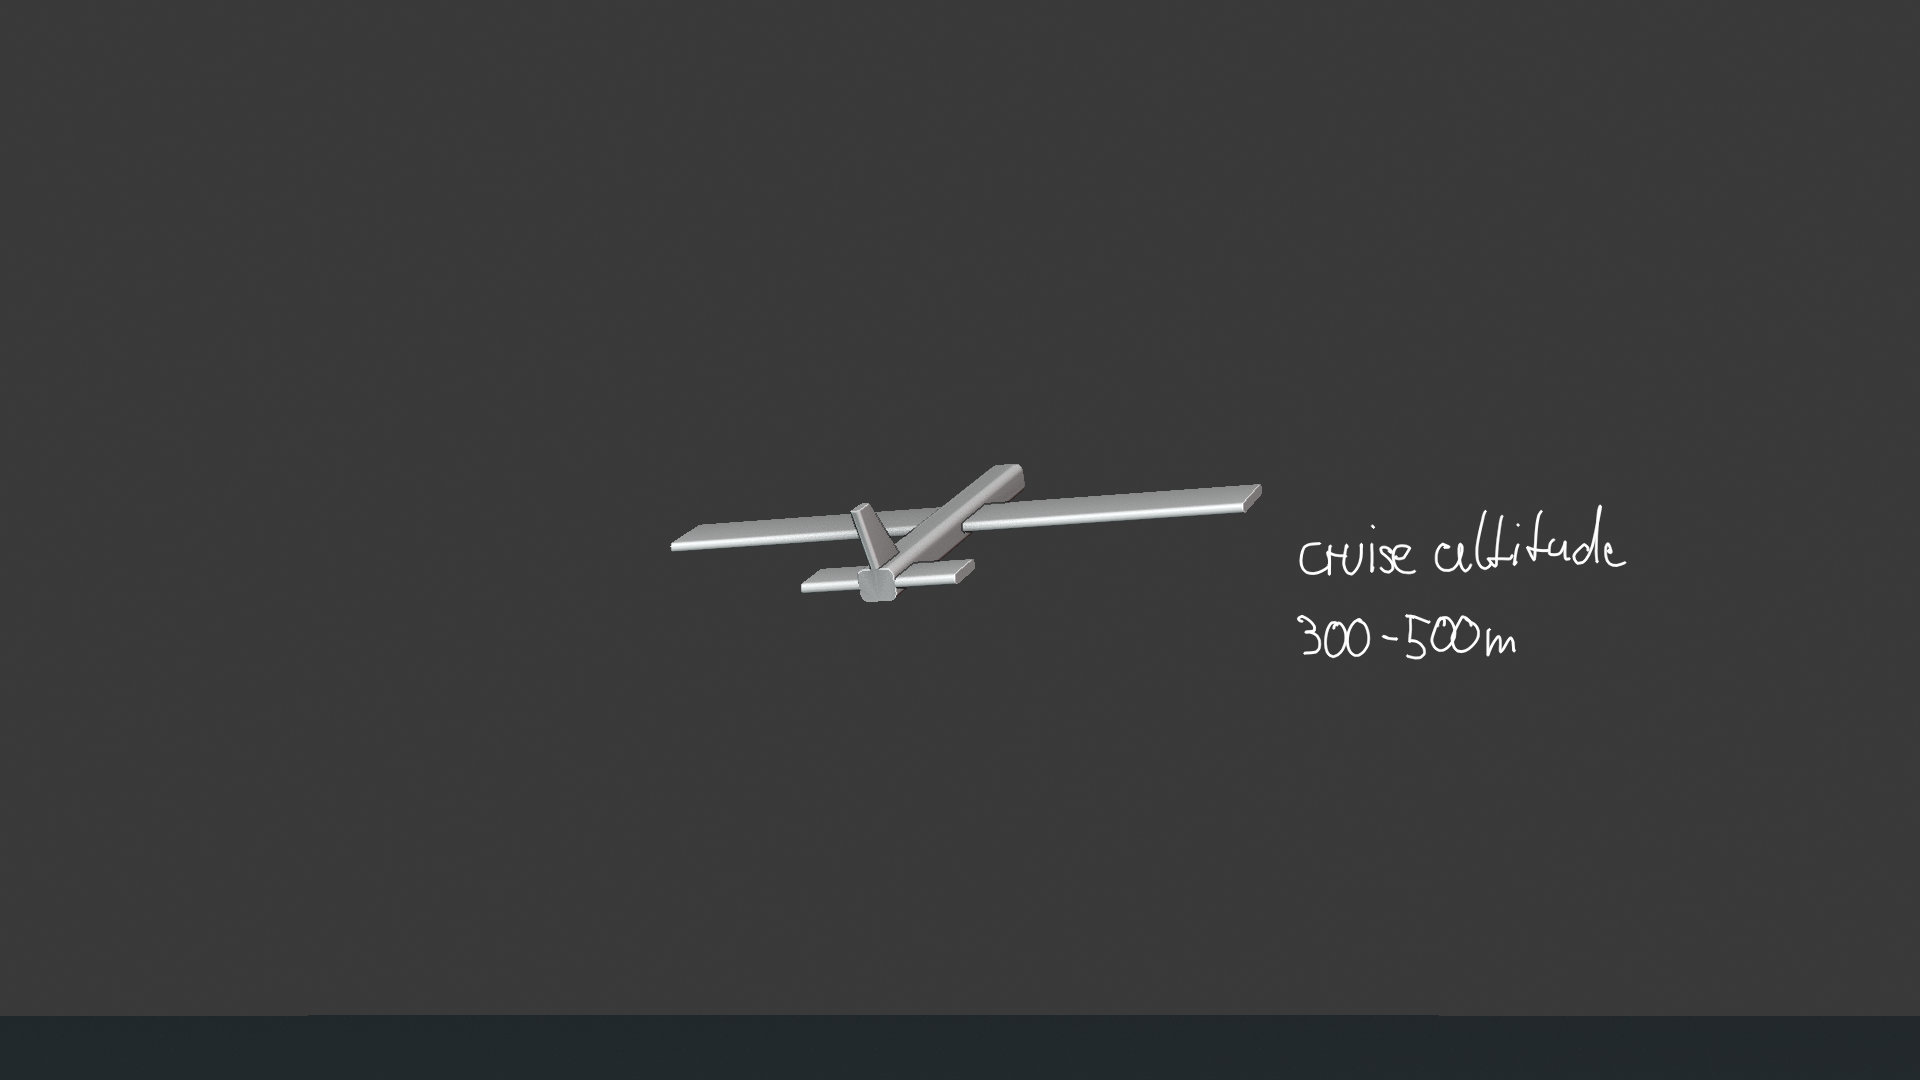
\includegraphics[width=\textwidth/2]{gfx/pre/0321.jpg}} \\
\subfloat[caption]{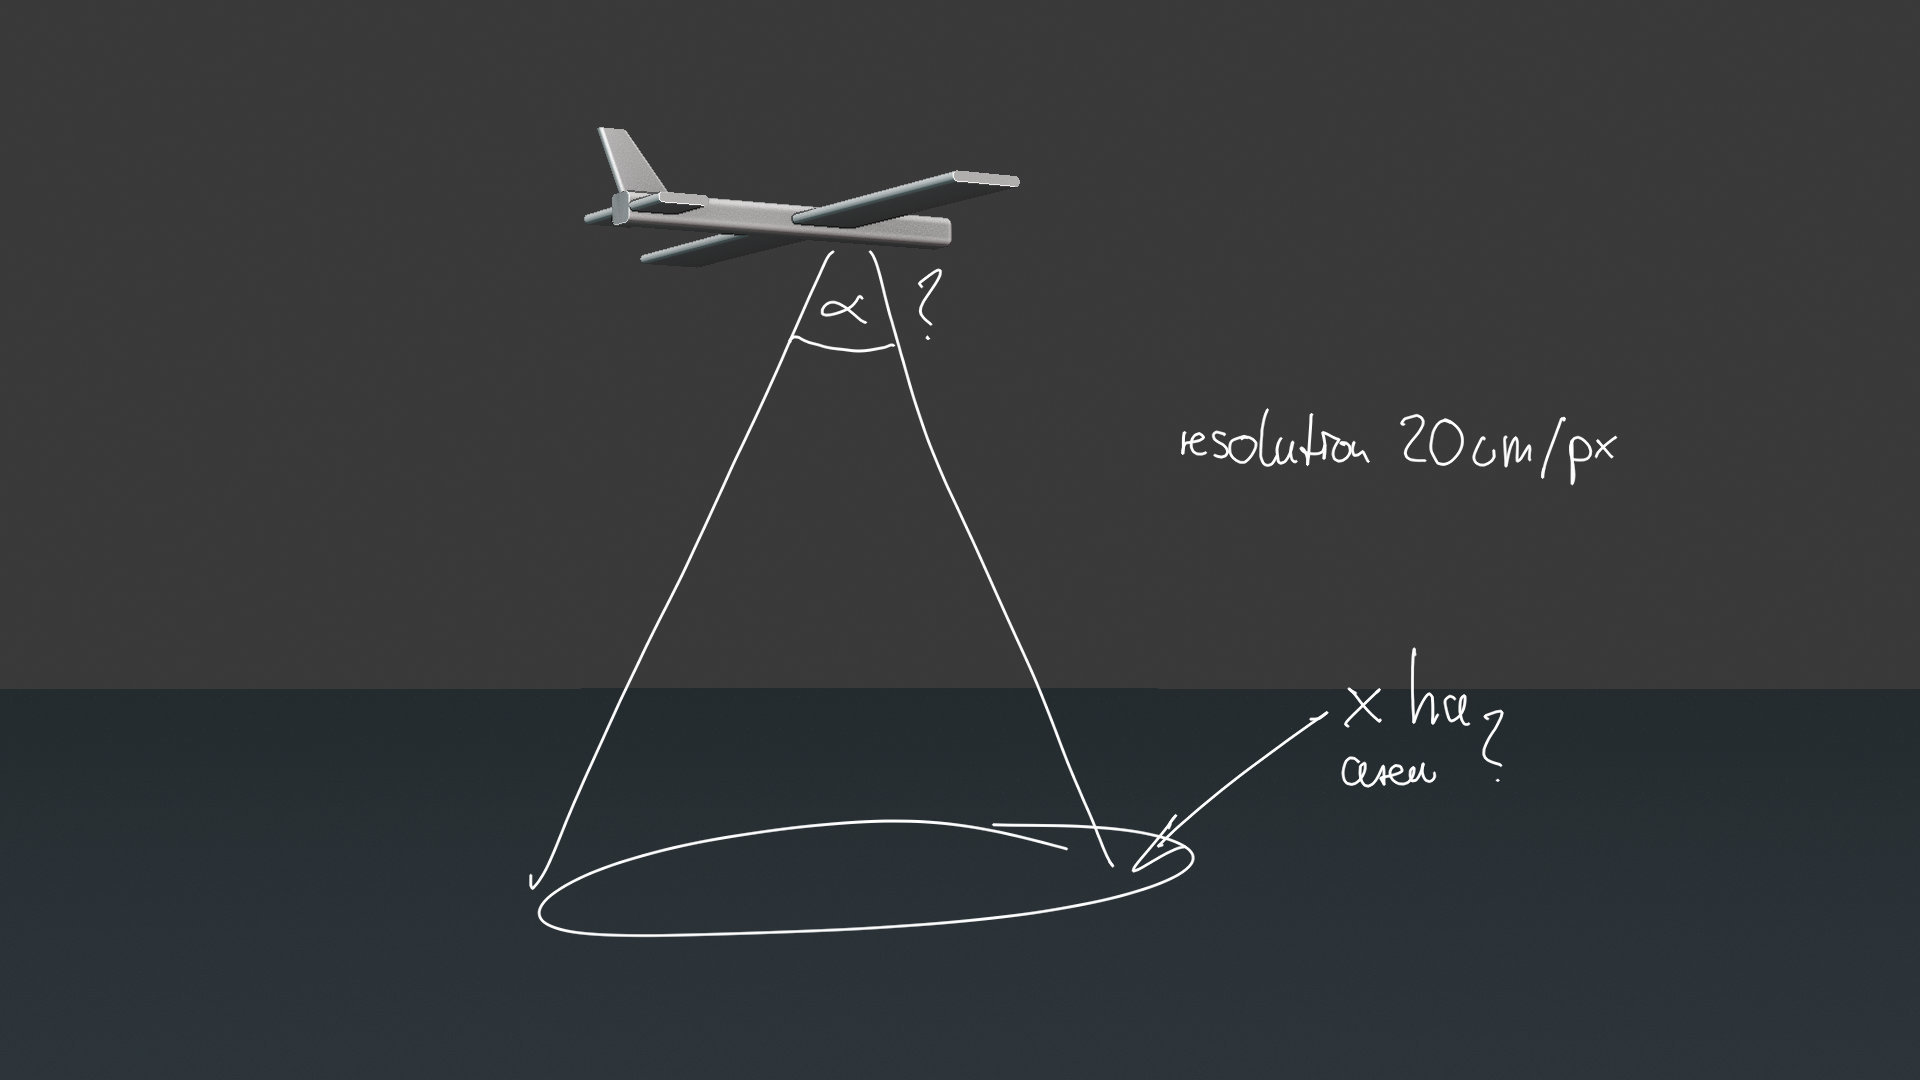
\includegraphics[width=\textwidth/2]{gfx/pre/0362.jpg}} &
\subfloat[caption]{
\includegraphics[width=\textwidth/2]{gfx/pre/0442.jpg}} \\
\subfloat[caption]{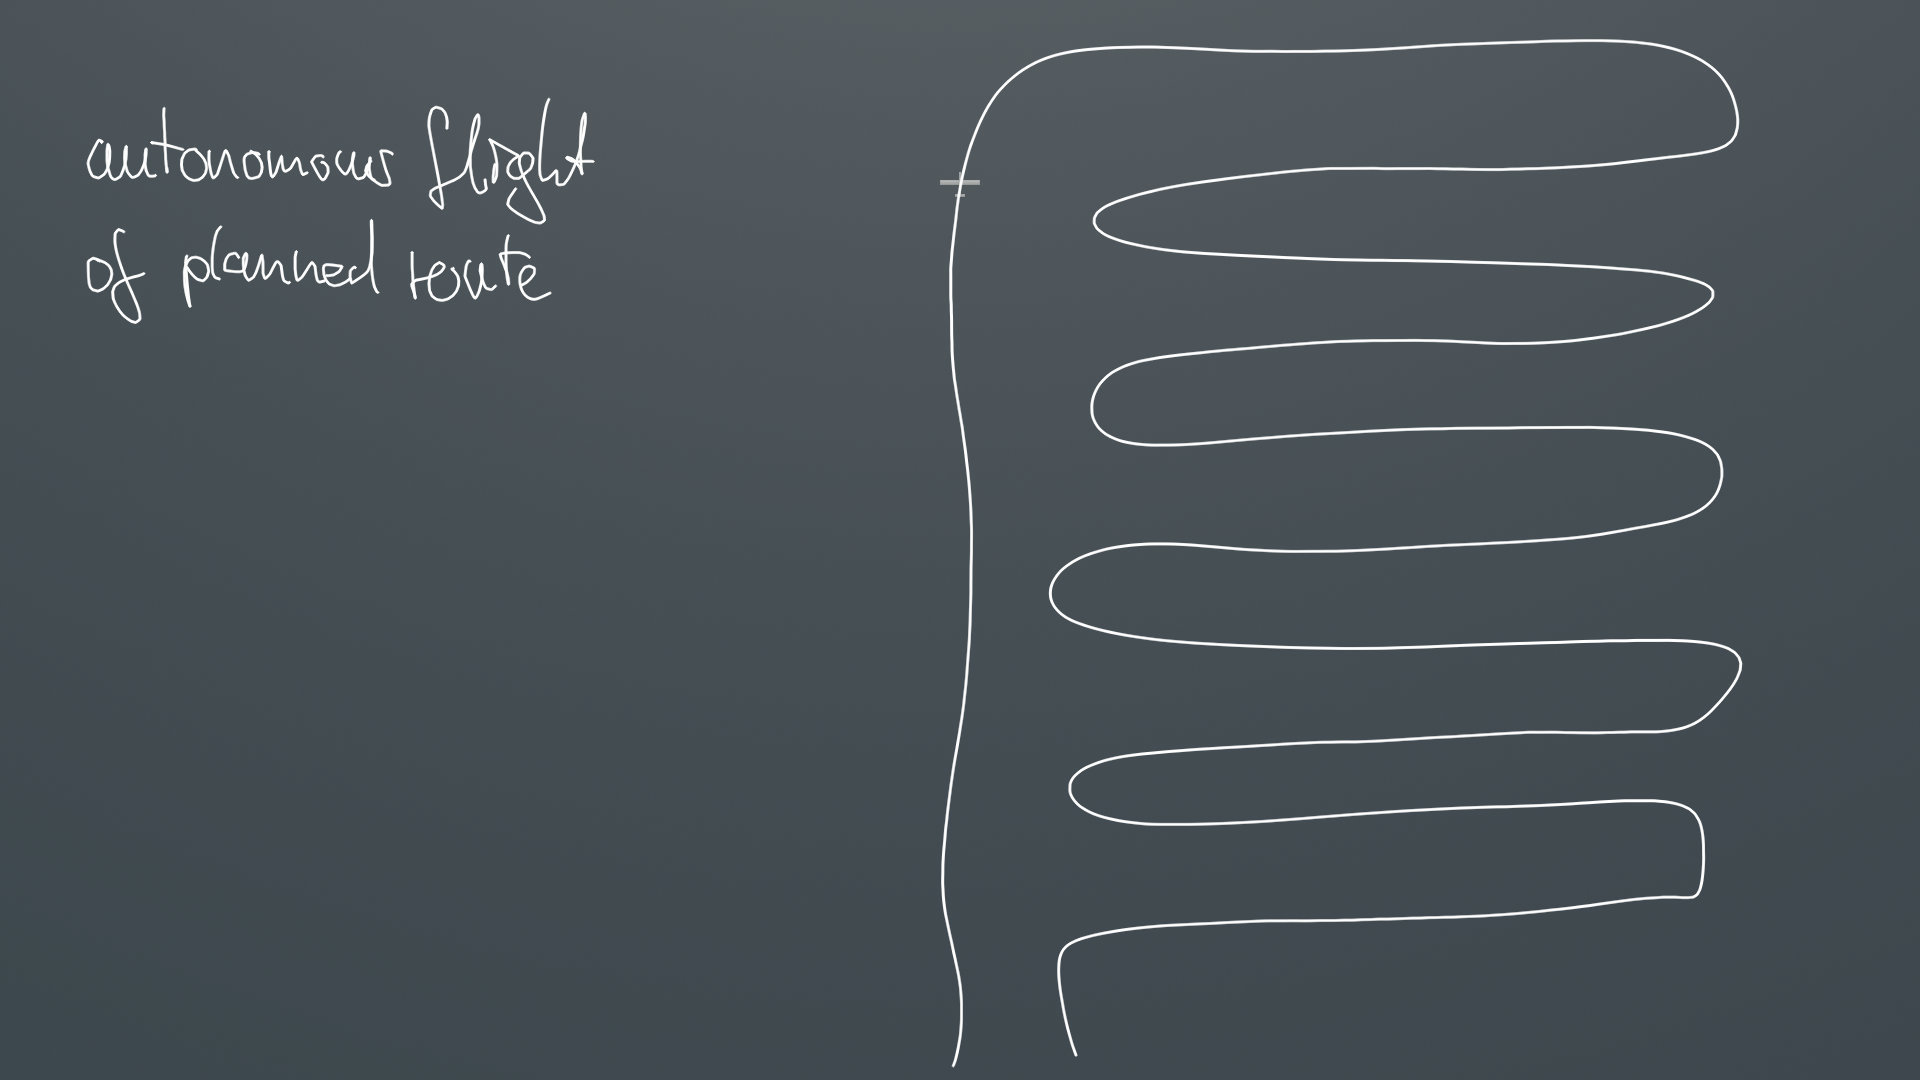
\includegraphics[width=\textwidth/2]{gfx/pre/0483.jpg}} &
\subfloat[caption]{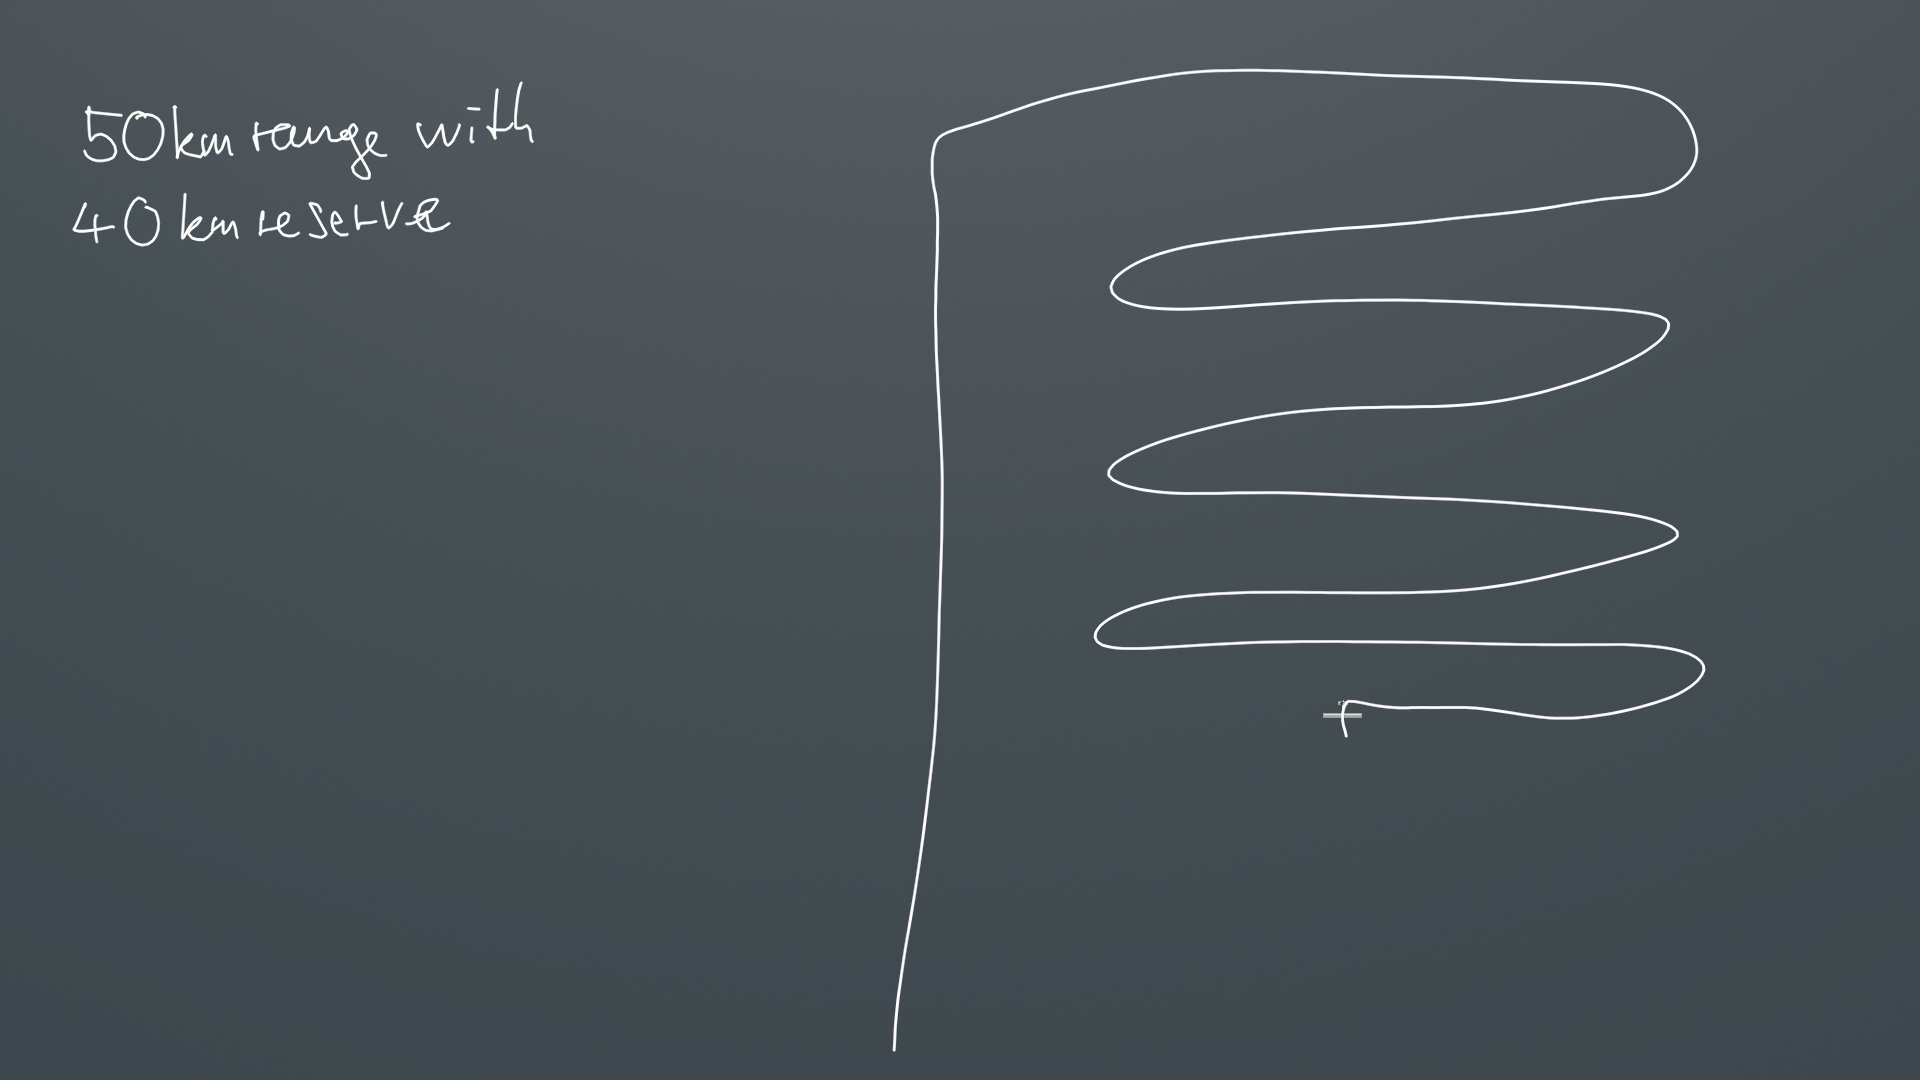
\includegraphics[width=\textwidth/2]{gfx/pre/0565.jpg}} \\
\subfloat[caption]{
\includegraphics[width=\textwidth/2]{gfx/pre/0606.jpg}} &
\subfloat[caption]{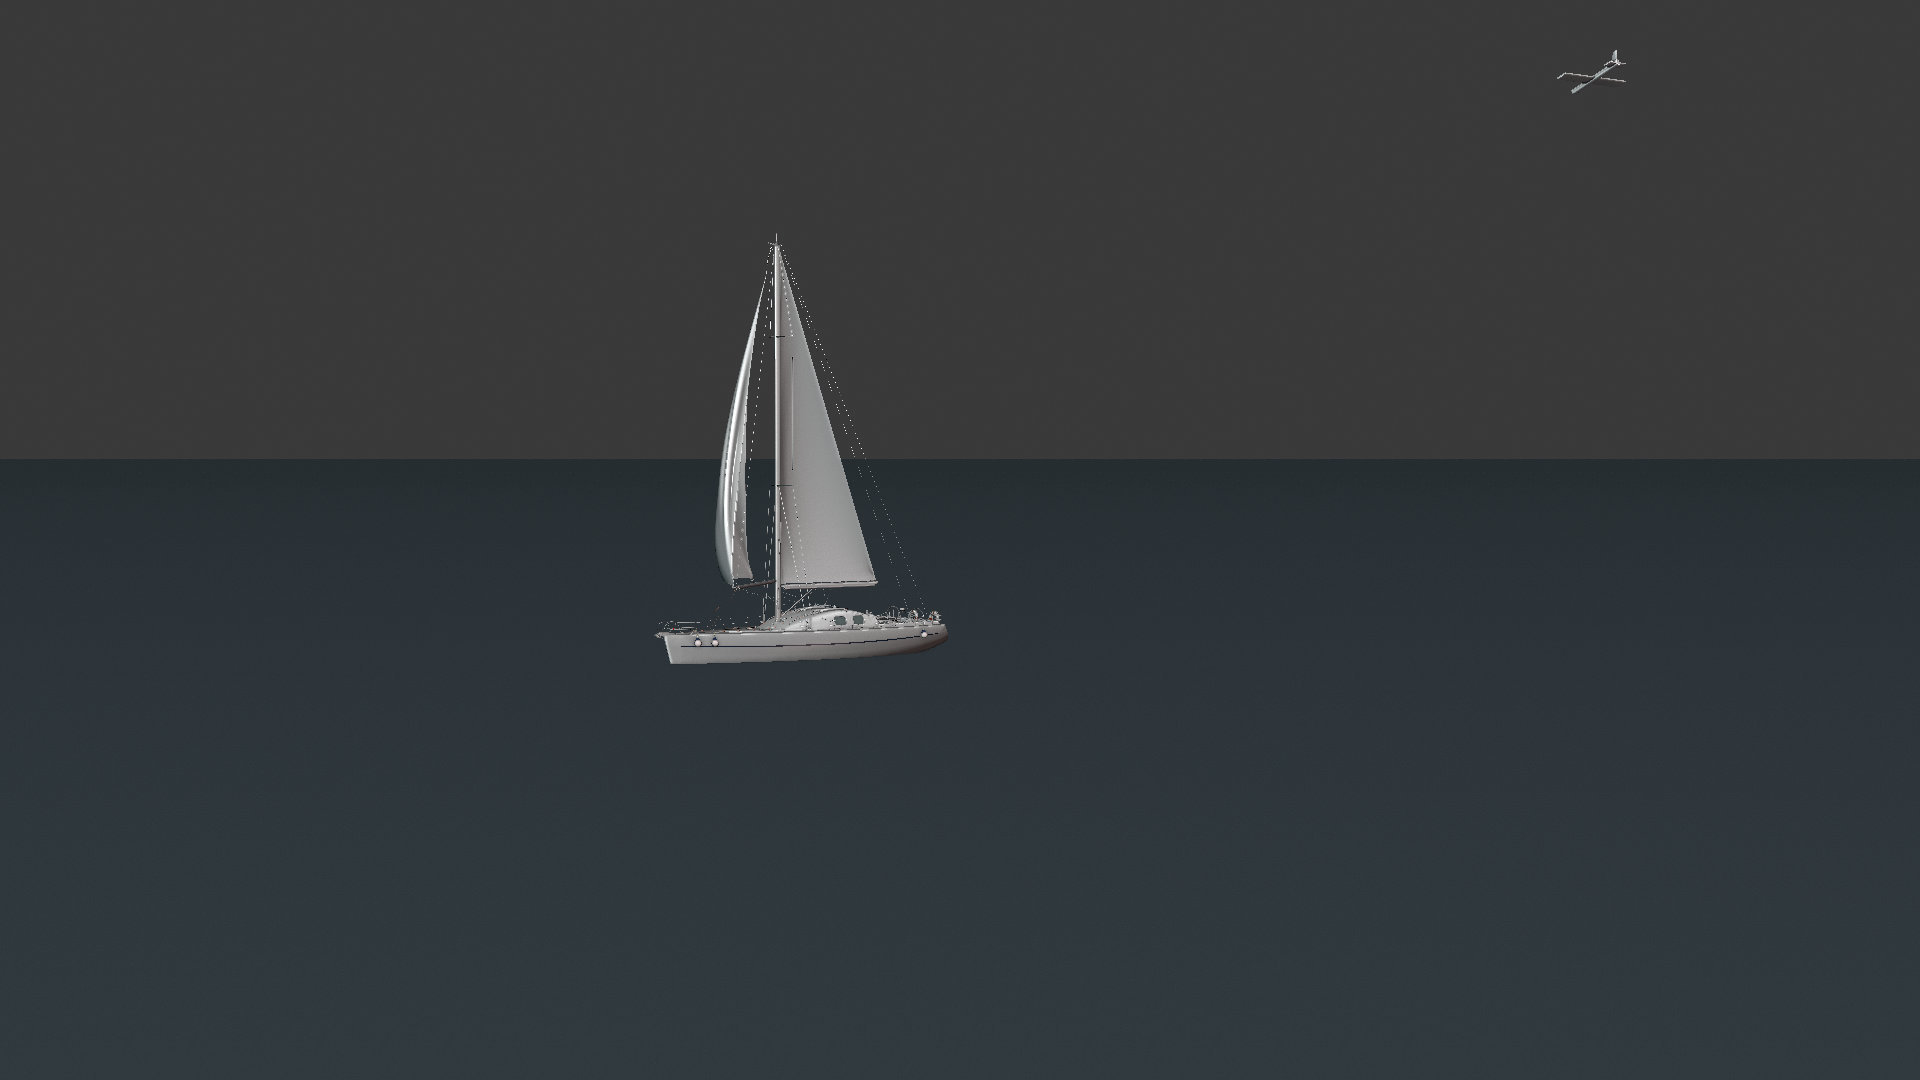
\includegraphics[width=\textwidth/2]{gfx/pre/0688.jpg}}
\end{tabular}
\end{figure}

